\chapter{数学环境}
\section{数学环境}
选择 \LaTeX 的一个很大的优势就是可以很好的输入数学公式, 下面是一些例子
\begin{theorem}
    这是一个定理
\end{theorem}
\begin{lstlisting}
    \begin{theorem}
        这是一个定理
    \end{theorem}
\end{lstlisting}

\begin{definition}
    这是一个定义
\end{definition}
\begin{lstlisting}
    \begin{definition}
        这是一个定义
    \end{definition}
\end{lstlisting}

\begin{corollary}
    这是一个推论
\end{corollary}
\begin{lstlisting}
    \begin{corollary}
        这是一个推论
    \end{corollary}
\end{lstlisting}

\begin{example}
    这是一个例子
\end{example}
\begin{lstlisting}
    \begin{example}
        这是一个例子
    \end{example}
\end{lstlisting}

\begin{proof}
    这是一个证明
\end{proof}
\begin{lstlisting}
    \begin{proof}
        这是一个证明
    \end{proof}
\end{lstlisting}

\section{公式测试}
行内公式 $ \lim_{x \to 0} \frac{\sin{x}}{x} = 1 $
\begin{lstlisting}
    行内公式 $ \lim_{x \to 0} \frac{\sin{x}}{x} = 1 $
\end{lstlisting}
行内公式行间表示 $ \displaystyle \lim_{x \to 0} \frac{\sin{x}}{x} = 1 $ 
\begin{lstlisting}
    行内公式行间表示 $ \displaystyle \lim_{x \to 0} \frac{\sin{x}}{x} = 1 $ 
\end{lstlisting}
无编号行间公式
\[  \lim_{x \to 0} \frac{\sin{x}}{x} = 1 \] 
\begin{lstlisting}
    \[  \lim_{x \to 0} \frac{\sin{x}}{x} = 1 \] 
\end{lstlisting}
有编号行间公式
\begin{equation}
    \lim_{x \to 0} \frac{\sin{x}}{x} = 1 
\end{equation}
\begin{lstlisting}
    \begin{equation}
        \lim_{x \to 0} \frac{\sin{x}}{x} = 1 
    \end{equation}
\end{lstlisting}
多行公式
\[
    \begin{aligned}
        x = & a+b+c+ \\
            & d+e+f+g
    \end{aligned} 
\]
\begin{lstlisting}
    \[
    \begin{aligned}
        x = & a+b+c+ \\
            & d+e+f+g
    \end{aligned} 
    \]
\end{lstlisting}
\section{浮动体测试}
不同于 Word 等排版引擎, \LaTeX 的特点是图表乱飞, 为此专门有人「搜索如何固定图表?」, 但这正是 \LaTeX 的优势, 图表会自动排版在合适的地方. 具有这种特性的环境, 在 \LaTeX 中称为「浮动体」. 一般条件下, 一页不要超过 5 个浮动体, 不然会发生浮动体冲突.
\subsection{图片测试}
测试图片 \ref{fig:myphoto}
\begin{figure}[htbp]
    \centering
    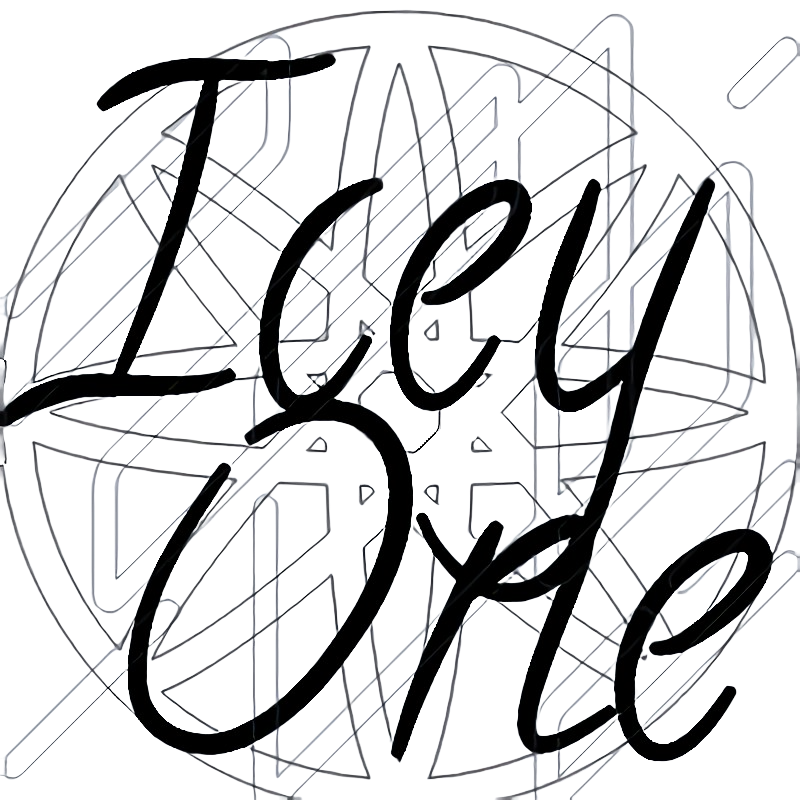
\includegraphics[width=\textwidth]{IceyOne.png}
    \caption{图片测试}
    \label{fig:myphoto}
\end{figure}
\begin{lstlisting}
    \begin{figure}[htbp]
        \centering
        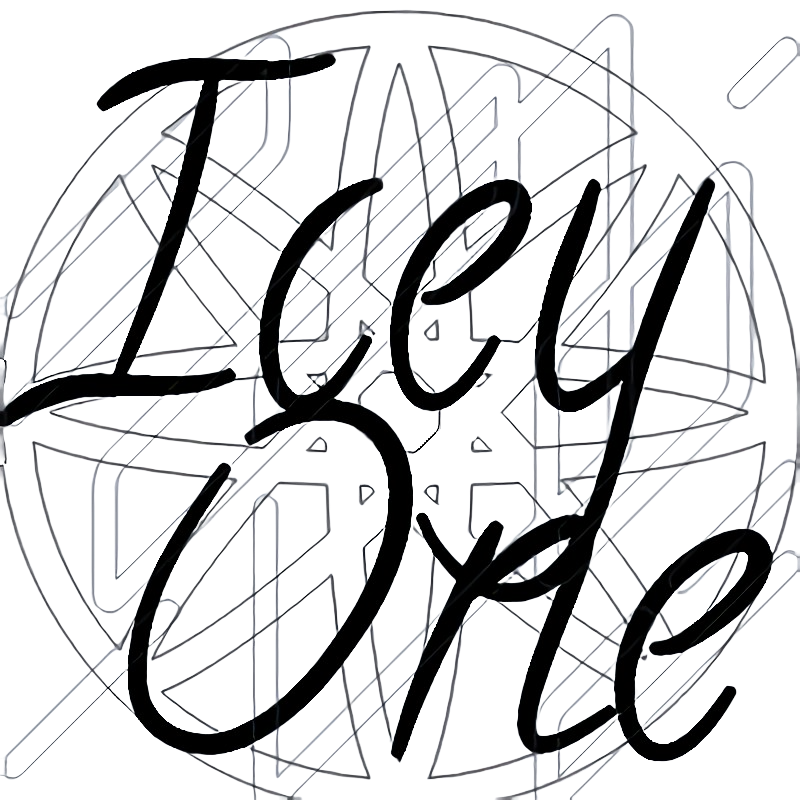
\includegraphics[width=0.10\textwidth]{IceyOne.png}
        \caption{图片测试}
        \label{fig:myphoto}
    \end{figure}
\end{lstlisting}
\subsection{表格测试}
如果对 \LaTeX 不太熟悉, 建议用 \href{https://www.tablesgenerator.com/}{Tables Generator} 或者 \href{https://tableconvert.com/}{Table Convert} 快速生成表格.
\begin{table}[htbp]
    \centering
    \caption{表格测试}
    \label{table:test}
    \begin{tabular}{llll}
        \hline
        Paremater & Markwodn & \LaTeX & Word \\ \hline
        上手难度 & 易 & 易 & 易 \\
        数学排版 & 支持 \LaTeX & 易 & 难 \\
        定制 & 易 & 很难 & 易 \\
        结构化 & 是 & 是 & 否 \\ \hline
    \end{tabular}
\end{table}
\begin{lstlisting}
    \begin{table}[htbp]
        \centering
        \caption{表格测试}
        \label{table:test}
        \begin{tabular}{llll}
            \hline
            Paremater & Markwodn & \LaTeX & Word \\ \hline
            上手难度 & 易 & 易 & 易 \\
            数学排版 & 支持 \LaTeX & 易 & 难 \\
            定制 & 易 & 很难 & 易 \\
            结构化 & 是 & 是 & 否 \\ \hline
        \end{tabular}
    \end{table}
\end{lstlisting}